\section{Théorie des Graphes}
\subsection{Introduction}
La théorie des graphes s'est développée au cours du \textsc{XX}\ieme siécle.
La génèse de la théorie des graphes semble être une étude de Léonard
\nom{Euler}, un très célèbre mathématicien du \textsc{XVIII}\ieme.
Dans un article publié en 1736, il traite un problème devenu classique,
illustré par la devinette : peut on faire une promenade passant une fois par
chacun des sept ponts de la ville de Koenigsberg?
Regardez la figure~\ref{fig.koenig}.
\begin{figure}
\centering
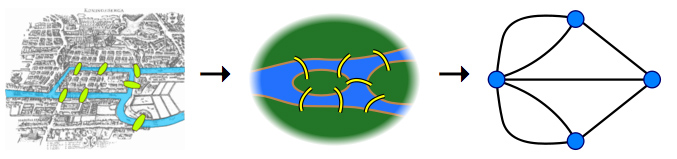
\includegraphics[width=0.8\textwidth]{koenigsberg}
\caption{Koenigsberg}\label{fig.koenig}
\end{figure}
\subsection{Les bases pour comprendre \algo}

\begin{defi}
  Un graphe $\Gamma(S, A)$ est la donnée de deux ensembles finis: un ensemble de
  sommets $S$ et un ensemble d’arêtes $A$. Une arête est une paire de sommets,
  ce sont les extrémités de l’arête. Une arête $\Set{x, y}$ est notée $xy$,
  et les sommets sont dits adjacents.
\end{defi}
\begin{defi}
  Un chemin de longueur n est une suite de  sommets $x_0, x_1, \dots , x_n$
  tels que :
  \[
  \forall i,\, 0 \leq i < n \implies x_i, x_{i+1} \in A
  \]
  Les sommets $x_0$ et $x_n$ sont les extrémités du chemin, $x_0$ est l’origine
et $x_n$ le sommet terminal. On parle de cycle quand $x_0 = x_n$. On dit
que $x$ est connecté à $y$, et on note $x \to y$ quand il existe un chemin
d’extrémité x et y. Il s’agit là d’une relation symétrique et transitive
qu’il convient de prolonger par réflexivité. Un chemin est dit simple
quand il ne passe jamais plus d’une fois par une même arête. Un chemin
élémentaire ne passe pas deux fois par un même sommet.
\end{defi}
\begin{defi}
L’ensemble des sommets voisins d’un sommet $x$ :
\[
\text{voisin($x$)} = \Set{ y \in S | xy \in A },\quad \text{deg($x$) = $\#$voisin($x$)}
\]
le degré d’un sommet est égal au nombre d’arêtes incidentes. Un
sommet de degré pair est dit pair, un sommet de degré impair est
dit impair.
\end{defi}
Nous avons l’amusante relation des paires et de l’impair
\begin{lemme}
  (parité et impairs). Dans un graphe, $\Gamma(S, A)$ :
  \[
  \sum_{x \in S} \text{deg($x$)} = 2 \lvert A \rvert
  \]
  en particulier, le nombre des sommets impairs est toujours pair.
\end{lemme}
\begin{proof}
  Notons $A_s$ les arêtes incidentes au sommet $s$,
  \[
  A = \bigcup_{s \in S} A(s).
  \]
Une triple intersection des $A_s$ est vide, une double intersection non
vide est une arête du graphe. Le principe d’inclusion et d’exclusion  s’applique sans difficulté et donne :
\[
\lvert A \rvert = \sum_{s \in S} \text{deg($s$)} - \lvert A \rvert
\]
\end{proof}
\begin{exo}
Prouver qu’un graphe d’ordre supérieur à 1, possède deux sommets de degré identique.
\end{exo}
\begin{exo}
 De tout parcours, on peut extraire un parcours élémentaire
ayant les mêmes extrémités. Détaillez cette affirmation !
\end{exo}
\begin{exo}
 Dans un graphe acyclique ayant au moins une arête, il existe un sommet de degré 1. Expliquez !
\end{exo}
Pour creuser plus sur l'intéresant théorie des graphes~\cite{langevin.book}.
